\documentclass{article}
\usepackage[utf8]{inputenc}
\usepackage[american]{babel}
\usepackage[T1]{fontenc}
\usepackage{amssymb,amsthm,amsmath,amsfonts}
\usepackage{algorithmic}
\usepackage{algorithm}
\usepackage{tikz}
\usepackage{nicefrac}
 
\newcommand{\todo}[1]{{\color{red}TODO: #1}}

\theoremstyle{plain}
\newtheorem{thm}{Theorem}
\newtheorem{lem}[thm]{Lemma}
\newtheorem{cor}[thm]{Corollary}
\newtheorem{prop}[thm]{Proposition}
\theoremstyle{definition}
\newtheorem{defi}[thm]{Definition}
\theoremstyle{remark}
\newtheorem{rem}[thm]{Remark}
\newtheorem{exe}[thm]{Example}

\title{Explicit isogenies in quadratic time in any characteristic}
\author{Cyril Hugounenq}

\begin{document}

\maketitle

\begin{abstract}
The problem we will consider here is the computation of an isogeny between two elliptics curves with the knowledge of the domain and the codomain of the isogeny and it's degree $r$. Couveignes's algorithm is an algorithm which solves this problem in $O(r^2)$ operations using the $p$-torsion. We want to extend the method used by Couveignes  We try to adapt his method here to the case of the $2$ torsion and more generally to the $\ell$ torsion, thus we propose an alternative for medium characteristic with this algorithm.
\end{abstract}

\section*{Proposed notation}

This section is for internal reference only: erase after the paper has
stabilized.

\begin{itemize}
\item $\mathbb{F}_q$ is the field we are working on
\item $\ell$ is for the $\ell$ torsion we are working on
\item $r$ is the degree of the isogeny we want to compute
\item $k$ is the integer such that $\ell^{2k}>4r+1$
\item we thus work with a tower which has for top level $F_{q^{\ell^k}}$
\item $E$ is for ordinary elliptic curves defined over the finite field $\mathbb{F}_q$
\item $\mathcal{O}$ (resp. $\mathcal{O}_x$) is the notation for the endomorphism ring associated (up to isomorphism) to $E$ (resp. $E_x$)
\item $K$ is the notation for the imaginary quadratic field in which $\mathcal{O}$ is defined
\item $d_K$ is the negative integer such that $K=\mathbb{Z}[d_K]$  
\end{itemize}

%%%%%%%%%%%%%%%

\section{Introduction}
\label{sec:introduction}

\todo{Isogenies of elliptic curves over finite fields are
  important. Isogenies are used in SEA. Isogenies are used in
  cryptography.  The \emph{explicit isogeny problem} is defined as
  follows\dots It is a fundamental subproblem in SEA. The best
  algorithms for it are\dots We present a quasi-quadratic-time
  algorithm working for finite fields of any characteristic, it is an
  alternative to the Lercier-Sirvent approach and compares favorably
  to it.}

% From a mail by Luca

% - Dans SEA, pour compter le nombre de points sur GF(p^n), on doit
% calculer des isogénies de degre ℓ~log(p^n).

% - Les algos classiques de calcul d'isogénies (CCR et BMSS) ratent dès
% que p >> ℓ.

% - Pour p fixé, on n'utilise pas SEA, mais plutôt les algos p-adiques.
% Ces algos sont exponentiels en log p.

% - Du coup, pour p pas fixé et n >> p/log(p) (carac moyenne), il y
% encore un intérêt à chercher des algos de calcul d'isogénies
% polynômiaux en log p.

% - Le seul algo de calcul d'isogénies qui marche pour tout p et qui
% n'est pas exponentiel en log p est Lercier-Sirvent. Il est quadratique
% en ℓ (plus le coût du polynôme modulaire, qui de toutes façons est
% déjà inclus dans SEA).

% Du coup, même si la carac moyenne n'est pas vraiment utilisée en
% crypto, ça reste intéressant de chercher des algos de calcul
% d'isogénie pour concurrencer Lercier-Sirvent.

The paper is organized as follows. In Section~\ref{sec:couv-algor} we
review Couveignes' strategy for the explicit isogeny problem, and
sketch our generalization of it. In
Section~\ref{sec:isogeny-volcanoes} we recall the fundamental
properties of isogenies and endomorphism
rings. Sections~\ref{sec:acti-frob-endm} and~\ref{sec:interpolation}
treat the two main phases of our new algorithm; both phases are used
together in Section~\ref{sec:complete-algorithm} to give the full
algorithm. Finally, Section~\ref{sec:implem} describes our
implementation of the algorithm and discusses its performances.


%%%%%%%%%%%%%%%

\section{Couveignes' algorithm}
\label{sec:couv-algor}

%Rappel sur l'algorithme de Couveignes, dire que basiquement il interpole un groupe de points sur un autre, puis fait de la reconstruction rationnelle et teste alors si son résultat est correct, si ce n'est pas le cas il change les groupes et recommence. 

Couveignes' algorithm \cite{couveignes96} is an algorithm which computes an isogeny using the $p$-torsion. This algorithm takes advantage of the cyclic group structure of the $p$ torsion to interpolate $p^k$ torsion points of one curve on another, with $k$ chosen such that $p^k>4r$. Couveignes's algorithm also take into account that if an isogeny send a point on an other then it also must respect the same property for the multiple points. With the interpolation polynomial Couveignes do a rational reconstruction of the isogeny, if the rational reconstruction don't work he tried with another couple of generators to do another interpolation. The complexity of this algorithm is of $O(r^2)$
\newline
We adapt his method here to the case of the $2$ torsion for ordinary elliptic curves and more generally to the $\ell$ torsion with $2 \wedge r ( \ell \wedge r)$.

Our goal is to reduce the number of points to interpolate with operations which are not so much costly. Thus we consider the Frobenius endomorphism to give us knowledge on the points we want to interpolate. We have considered the graph of isogeny (called volcano) which is linked to the group structure (see \cite{MiretMRV05}, \cite{IonicaJ10} ) of the curve for our study. First we have to determined which knowledge we obtain thanks to the Frobenius. The Frobenius allow us to determine horizontal isogenies according to the "notations" from \cite{Kohel} and \cite{volcano}, and thus we can associate to those horizontal isogenies their kernel and then one generator of their kernel. It will be those generators that we will use for the interpolation. To speed up the interpolation computation we will use techniques such as one used in \cite{enge+morain03} where we take into account the action of the Frobenius. In the end we will obtain a computational complexity of $O(r^2)$.

%%%%%%%%%%%%%%%

\section{Isogeny volcanoes}
\label{sec:isogeny-volcanoes}

\todo{Notions de base sur les isogenies et les volcans.}

%Dire que le volcan ne possède des isogenies

%%%%%%%%%%%%%%%

\section{The action of the Frobenius endmorphism}
\label{sec:acti-frob-endm}
\todo{Dans cette section on montre les résultats que nous permettent d'obtenir le frobenius sur le cratère}
To be able to distinguish two different horizontal isogenies and the descending ones on the crater of the volcano, we need the Frobenius to have two distincts eigenvalues which is only possible on the cyclic crater of a volcano of $\ell$-isogeny.

\begin{prop}
For $\lambda_1 , \lambda_2$ the $2$ eigenvalues of the Frobenius and $k>\nu_2(\lambda_1-\lambda_2)$, the matrix of the Frobenius action on the $\ell^k$ torsion is only diagonalisable on a cyclic crater of a volcano of $\ell$ isogeny.
\end{prop}

\begin{proof}
We remind that with the notation from \cite{Fouquet01} \cite{Kohel96} we have $d_{\pi}=g^2d_K$, with $d_K$ squarefree.
\newline
If we have $\left( \frac{d_K}{\ell} \right)=1$ then we have $x^2 = d_K \bmod \ell$ who has a solution so the characteristic polynomial of the Frobenius has two roots in $\mathbb{Z}_{\ell}$. If $\left( \frac{d_K}{\ell} \right)=-1$ then we have $x^2 = d_K \bmod \ell$ who has no solution so the characteristic polynomial of the Frobenius has no roots in $\mathbb{Z}_{\ell}$. If $\left( \frac{d_K}{\ell} \right)=0$ thus we have $x^2 = d_K \bmod \ell$ who has the trivial solution so the characteristic polynomial of the Frobenius has a unique root in $\mathbb{Z}_{\ell}$.
\newline
We thus work with $\left( \frac{d_K}{\ell} \right)=1$. We are obliged to work in $\mathcal{O}_K$ (crater)  because the eigenvalues of the Frobenius are not defined in $\ell \mathcal{O}_K$ since $\sqrt{d_K}$ is not.
\end{proof}

From this point we study the $\ell$ torsion points who are eigenvector for the Frobenius, thus we work with curves who are on the cyclic crater of a volcano (i.e. when $\left( \frac{d_K}{\ell} \right)=1$). We have to determine  the two eigenvalues of the Frobenius and $2$ points of $\ell^{\nu_{\ell}(\lambda_1-\lambda_2)+1}$ order who are also eigenvector for the $2$ eigenvalues. We use the following algorithm to do so. This algorithm computes a diagonalized basis of the $\ell^{s+1}$ torsion for the Frobenius from the knowledge of $\lambda_1, \lambda_2 \bmod \ell^s$ and a diagonalized basis of the $\ell^s$ torsion for the Frobenius. We do this for $s=1$ to $s=k$.
%First we have to tell how we obtain such a basis and the eigenvalues
\begin{algorithm}
\caption{\label{Diagnoalizedbasis}Diagonalizing and computing the basis $\langle P,Q \rangle $ of the $\ell^k$ torsion.}
\begin{algorithmic}[5]
\REQUIRE $\langle P,Q \rangle$ a basis of the $\ell$-torsion.
\ENSURE $\langle P,Q \rangle$ a basis of the $\ell^k$-torsion, $\lambda_1, \lambda_2$ defined modulo $\ell^k$ such that $\pi(P)=\lambda_1P$, $ \pi(Q)=\lambda_2Q$
\STATE $h:=1, k_0:=1$
\FOR {$i=1$  to  $k-1$}
\STATE $P \leftarrow P/\ell$
\STATE $Q \leftarrow Q/\ell$ 
\STATE compute $\pi(P,Q)=\left( \begin{array}{cc}
\lambda_1 + a\ell^{i} & b\ell^{i}\\
c\ell^{i} & \lambda_2 + d\ell^{i}
\end{array} \right) \bmod \ell^{i+1}$ with $\{a,b,c,d\} \in \mathbb{Z}/\ell\mathbb{Z}$
\IF {$\lambda_1 \neq \lambda_2$}
\STATE $k0 \leftarrow \frac{\lambda_1-\lambda_2}{\ell^h}$
\ENDIF
\STATE $\lambda_1, \lambda_2  \gets \lambda_1 + a\ell^i, \lambda_2 + d\ell^i$
\STATE $r_1,r_2 \gets \frac{-b }{k_0}, \frac{c }{k_0}$  
\STATE $\{P,Q\} \gets \{P+\ell^{i-1-h}r_1Q,Q+\ell^{i-1-h}r_2P\}$
\IF {$\lambda_1 = \lambda_2$}
\STATE $h \leftarrow h+1$
\ENDIF
\ENDFOR
\RETURN $\{P,Q,\lambda_1,\lambda_2\}$
\end{algorithmic}
\end{algorithm}


To distinguish the two eigenvalues of the Frobenius we are forced to consider the $\ell^k$ torsion for $k>\nu_{\ell}(\lambda_1-\lambda_2)$. We obtain the following result who link the $\ell$ isogenies and the $\ell^k$ torsion points.

\begin{prop} \label{conjecture}
For $P$ a point of order $\ell^{\nu_{\ell}(\lambda_1-\lambda_2)+1}$ on $E$ which is on a cyclic crater, with $\lambda_1, \lambda_2$ the two eigenvalues associated to $\pi$, then
\begin{itemize}
\item Either $\pi(P)=\lambda_1P$ then the $\ell$-isogeny with kernel $\ell^{\nu_{\ell}(\lambda_1-\lambda_2)} P$ is horizontal,
\item Either $\pi(P)=\lambda_2P$ then the $\ell$-isogeny with kernel $\ell^{\nu_{\ell}(\lambda_1-\lambda_2)} P$ is horizontal,
\item or $\pi(P) \neq \lambda_2P$ and $\pi(P) \neq \lambda_1P$ then the $\ell$-isogeny with kernel $\ell^{\nu_{\ell}(\lambda_1-\lambda_2)} P$ is descending.
\end{itemize} 
\end{prop}

\begin{proof}
We denote by $h$ the value $\nu_{\ell}(\lambda_1-\lambda_2)$ and  $Es_1=\{P \in E[\ell^h], \ell^{h-1}P \neq 0, \pi(P)=\lambda_1P\}$, $Es_2=\{P \in E[\ell^h], \ell^{h-1}P \neq 0, \pi(P)=\lambda_2P\}$ and consider $\phi_1$(resp. $\phi_2$) the $\ell$isogeny generated by $Es_1$ (resp. $Es_2$). This isogeny is unique since those eigenspace are of dimension $1$. % on pourrait se passer de cette dernière phrase... 
We consider the notations from the complex multiplication theory with $K$ the quadratic imaginary field which contains the endomorphism ring of $E$: $\mathcal{O}$. In particular, with the notation of $\mathcal{O}_K$ for the algebraic integers of $K$ we have $[\mathcal{O}:\mathcal{O}_K]\wedge \ell =1$, since we have a cyclic crater $\left( \frac{d_K}{\ell} \right)=1$ then (by Proposition 5.11 of \cite{Cox89} )  $p\mathcal{O}_K=\mathfrak{p}_1\mathfrak{p}_2\mathcal{O}_K$ with $Gal(K/\mathbb{Q})$ such as $\mathfrak{p}_1'=\mathfrak{p}_2$ (by theorem 5.9 of \cite{Cox89}). Since $Es_1$ and $Es_2$ are also conjugated with $Gal(K/\mathbb{Q})$ we can associate to the isogeny $\phi_1$ (resp. $\phi_2$)  the integral ideal $\mathfrak{p}_1\mathcal{O}_K$ (resp. $\mathfrak{p}_2\mathcal{O}_K$) and the endomorphism ring $\mathfrak{p}_1^{-1}\mathcal{O}_K$ (resp. $\mathfrak{p}_2^{-1}\mathcal{O}_K$) to their codomain. Since we got $\mathfrak{p}_1\mathfrak{p}_2=p$ then $\mathfrak{p}_1^{-1}=\left( \frac{\mathfrak{p}_2}{p} \right)$ therefore $[\mathcal{O}_K:\left( \frac{\mathfrak{p}_2}{p} \right)\mathcal{O}_K]\wedge \ell =1$. The others isogenies are those associated to the integral ideals $a  \mathfrak{p}_1 + \mathfrak{p}_2$ with $a \wedge \ell =1$ and to the groups which are generated by a linear combination of points of $Es_1$ and $Es_2$
\end{proof}


\subsection{Horizontal basis}
\todo{Dans cette section on montre comment on construit une base horizontale de la $2(\ell)$ torsion}
Our aim now is to compute  a basis of the $\ell^{\nu_{\ell}(\lambda_1-\lambda_2)+1}$ torsion with each generator who is also a generator of a $\ell^{\nu_{\ell}(\lambda_1-\lambda_2)+1}$ horizontal isogeny, but first we have to define them:

\begin{defi}%peut etre que le choix du r est malheureux dans cette definition...
Let $\phi$ be a $\ell^r$-isogeny with $r>0$, we say that $\phi$ is horizontal  if there exists a decomposition $\phi = \psi_1 \circ … \circ \psi_r$, where all $\ell$-isogenies $\psi_i$ are horizontal.
\end{defi}

To compute such a basis we start from a basis of the $\ell^{\nu_{\ell}(\lambda_1-\lambda_2)+1}$ torsion of a curve on a cyclic crater of the $\ell$ isogeny volcano and then we push this basis along the crater thanks to the knowledge from the Frobenius.

\begin{prop}\label{propcentrale}
Let $E$ be an elliptic curve over a cyclic crater of a volcano of $\ell$-isogenies, we consider a  point of order (at least) $\ell^{\nu_{\ell}(\lambda_1-\lambda_2)+1}$ $Q \in E$ such that $\varphi: E \rightarrow \nicefrac{E}{\langle Q \rangle }$ is a horizontal isogeny and $\pi(Q)=\lambda_2(Q)$, $P$ a point of $\ell^{\nu_{\ell}(\lambda_1-\lambda_2)+1}$ order such that $\pi(P) = \lambda_1P$. We denote by $\phi$ the isogeny: $E\rightarrow E^*=\nicefrac{E}{\langle P \rangle}$. For $R$ a $\ell$ division point of $Q$ we have $\phi(R)$ such that $E^* \rightarrow \nicefrac{E^*}{\langle \phi(R) \rangle}$ is a horizontal isogeny.  
\end{prop}

\begin{figure}
\begin{center}
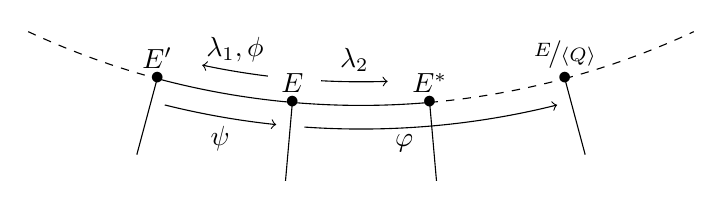
\begin{tikzpicture}[scale=1]
\coordinate (A) at (245:10);
\coordinate (B) at (255:10);
\coordinate (B') at (255:11);
\coordinate (B1) at (256:10.3);
\coordinate (C) at (265:10);
\coordinate (C') at (265:11);
\coordinate (D) at (275:10);
\coordinate (D') at (275:11);
\coordinate (E) at (285:10);
\coordinate (E') at (285:11);
\coordinate (F) at (295:10);
\coordinate (F') at (295:11);
\coordinate (G) at (305:10);
\coordinate (B2) at (258:9.7);
\coordinate (C1) at (266:10.3);
\coordinate (C2) at (267:9.7);
\coordinate (encre) at (273:10.5);
\draw (A) arc(245:255:10)[dashed];
\draw (B) arc(255:275:10);
\draw (D) arc(275:285:10)[dashed];
\draw (E) arc(285:295:10)[dashed];
\draw (B) node[above] {$E'$} node{$\bullet$};
\draw (C) node[above] {$E$} node{$\bullet$};
\draw (D) node[above] {$E^*$} node{$\bullet$};
\draw (E) node[above] {$\nicefrac{E}{\langle Q \rangle }$} node{$\bullet$};
\draw (encre) node {$\varphi$};
\draw (B)--(B');
\draw (C)--(C');
\draw (D)--(D');
\draw (E)--(E');
\draw (B1) arc(256:264:10.3) [->] node[below,midway] {$\psi$}; %flèche représentant \psi
\draw (B2) arc(258:263:9.7) [<-] node[above,midway] {$\lambda_1, \phi$}; %flèche représentant 
\draw (C2) arc(267:272:9.7) [->] node[above,midway] {$\lambda_2$}; %flèche représentant 
\draw (C1) arc(266:284:10.3) [->];% node[below,midway,fill=white] {$\varphi $};

%\draw (260:10.75) node{}
%\draw (0,0) arc (245:255:10)[dashed] node[above] {$C$} node{$\bullet$} --(0:1.5);
%\draw (0,0) arc (245:255:10)[dashed] arc (255:265:10) node[above] {$E^i$} node{$\bullet$} --(0:1.5);
%\draw (-1,0) arc (245:255:10) node[above] {$C2$} node{$\bullet$} --(90:1)[color=yellow];
%\draw (-1,0) arc (245:255:10) node[above] {$C$} node{$\bullet$} --(310:1.5)[color=red];
%\draw (0,0) arc (245:255:10)[color=white] node[above] {$C$} node{$\bullet$} arc (255:265:10) node[above] {$E^i$} node{$\bullet$} arc (265:275:10) node[above] {$E$} node{$\bullet$} arc (275:285:10) node[above] {$F$} node{$\bullet$} arc (285:295:10) node[above] {$G$} node{$\bullet$} ; 
\end{tikzpicture}
\end{center}
\caption{ Example for the case $\ell=2$ } 
\end{figure}

\begin{proof}
We will first prove that the isogeny $E^* \rightarrow \nicefrac{E^*}{\phi(R)}$ is horizontal and associated to $\lambda_2$.
\newline
The $\ell$ adic valuation of the order of $Q$ is denoted by $d_Q$. Since $\ell \pi(R)=\pi(Q)=\lambda_2Q$ then the $\ell$-isogeny $\psi$ with kernel $\ell^{d_Q}\phi(R)$ is the dual isogeny of $\phi$ because it is the one who anhiliates the $\ell$-torsion (here $\langle P, \ell^{d_Q-1}Q \rangle$) together with $\phi$ on $E$. Thus we have proved that $\psi$ is associated to $\lambda_2$ and horizontal. 
\newline
Since we have $\psi(\phi(R))=Q$, this tells us that the isogeny $\Upsilon$ with kernel $\phi(R)$ is the composition of $\psi$ with the isogeny $\varphi$ of kernel $\langle Q \rangle$. Thus the isogeny $\Upsilon$ is horizontal of degree $\ell^{d_Q+1}$ and associated to $\lambda_2$. 
\end{proof}

%Algorithme necessaire, surement pour enfoncer le clou...

\subsection{Proof of the algorithm}
\todo{Dans cette section on montre que une base horizontale est envoyee sur une base horizontale}
Now that we have seen a way to determine a set of $\ell^{\nu_{\ell}(\lambda_1-\lambda_2)+1}$ torsion points, we have to show that this set is invariant under isogenies of degree prime to $\ell$.

\begin{prop}
Let $Q$ be a point of $\ell^j$ torsion with $j>0$ then there exists a division point $R$ of $Q$ of order $\ell^{h+j}$ with $\pi(R)=\lambda_2R$ if and only if the $\ell^j$ isogeny with kernel $\langle Q \rangle $ is horizontal.
\end{prop}

\begin{proof}
In \ref{propcentrale}, the $\Leftarrow$ has NOT been proved. Now we will prove the other way.
\newline
We do a recursive proof. The initial step is the conjecture \ref{conjecture}.
\newline
Recursive step: we consider that the property is true to the rank $j>1$, then we will have to prove it for $j+1$.
We consider then $S$ a point of order $\ell^{j+1}$ with $T$ a division point of $S$ of order $\ell^{h+1+j}$ with $\pi(T)=\lambda_2T$.We know that the $\ell^j$ isogeny $\phi$ generated by $\langle \ell S \rangle$ is horizontal and associated to $\lambda_2$. We then have $\phi(S)$ a point of order $\ell$ and $\phi(T)$ a point of order $\ell^{h+1}$ with $\pi(\phi(T))=\lambda_2\phi(T)$. Thus by applying the conjecture \ref{conjecture} we have the isogeny $\psi$ with kernel $\langle \phi(S) \rangle$ horizontal, therefore the isogeny with kernel $\langle S \rangle$ who is equal to the composition of $\psi$ with $\phi$ is horizontal.
\end{proof}

\begin{prop}
For $\phi$: $E \rightarrow E'$ a $r$-isogeny  with $r \wedge \ell=1$ an odd prime, and $P$ a $\ell^i$ primitive torsion point, with $i>0$ such that $E \rightarrow E / \langle P \rangle $ is horizontal and $P$ is associated to $\lambda_1$. Then the isogeny  $E' \rightarrow E' / \langle \phi(P) \rangle$ is also horizontal.
\end{prop}

\begin{proof}
We just have to prove that there exists a $\ell^{h+i}$ primitive torsion point $V$ dividing $\phi(P)$ such that $\pi(V)=\lambda_1P$.
Since $P$ is a point that generates a horizontal isogeny then there exists a point $R$ of order $\ell^{h+i}$ dividing $P$. Since $\phi$ is a $r$ isogeny then $\phi$ doesn't change the order of $P$ and $R$, moreover the frobenius commutes with $\phi$ (because this one is defined on $\mathbb{F}_q$) then we have $\pi(\phi(R))=\lambda_1\phi(R)$ which proves the assertion.
\end{proof}

%%%%%%%%%%%%%%%

\section{Interpolation step}
\label{sec:interpolation}
\todo{Dans cette section on montre les outils employes pour diminuer le cout de l interpolation}

%%%%%%%%%%%%%%%

\section{Complete algorithm}
\label{sec:complete-algorithm}
\todo{Put pieces together: explain the strategy for the case where the
  curves are not on the crater, characterize cases where the algorithm
  works/doesn't work, state overall complexity.}

%%%%%%%%%%%%%%%

\section{Experimental results}
\label{sec:implem}

\todo{Describe implementation and show benchmarks. Possibly compare
  with Lercier-Sirvent (Luca has an implementation somewhere).}

\bibliographystyle{plain}
\bibliography{refs}

\end{document}
